\chapter[Models]{Physical and numerical models}

\section{Physical and mathematical description} 

Characteristic of compositional multiphase models is that the phases
are not only matter of a single chemical substance. Instead, their
composition in general includes several species, and for the mass transfer, 
the component behavior is quite different from the phase behavior. In the following, we
give some basic definitions and assumptions that are required for the
formulation of the model concept below. As an example, we take a
three-phase three-component system water-NAPL-gas
\cite{A3:class:2002a}. The modification for other multicomponent
systems is straightforward and can be found, e.\ g., in
\cite{A3:bielinski:2006,A3:acosta:2006}.

\subsection{Basic Definitions and Assumptions for the Compositional
  Model Concept}
\textbf{Components:}
The term {\it component} stands for constituents of the phases which
can be associated with a unique chemical species, or, more generally, with 
a group of species exploiting similar physical behavior. In this work, we
assume a water-gas-NAPL system composed of the phases water (subscript
$\text{w}$), gas ($\text{g}$), and NAPL ($\text{n}$). These phases are
composed of the components water (superscript $\text{w}$), air
($\text{a}$), and the organic contaminant ($\text{c}$) (see Fig.\
\ref{A3:fig:mundwtrans}).
%
\begin{figure}[hbt]
  \centering
  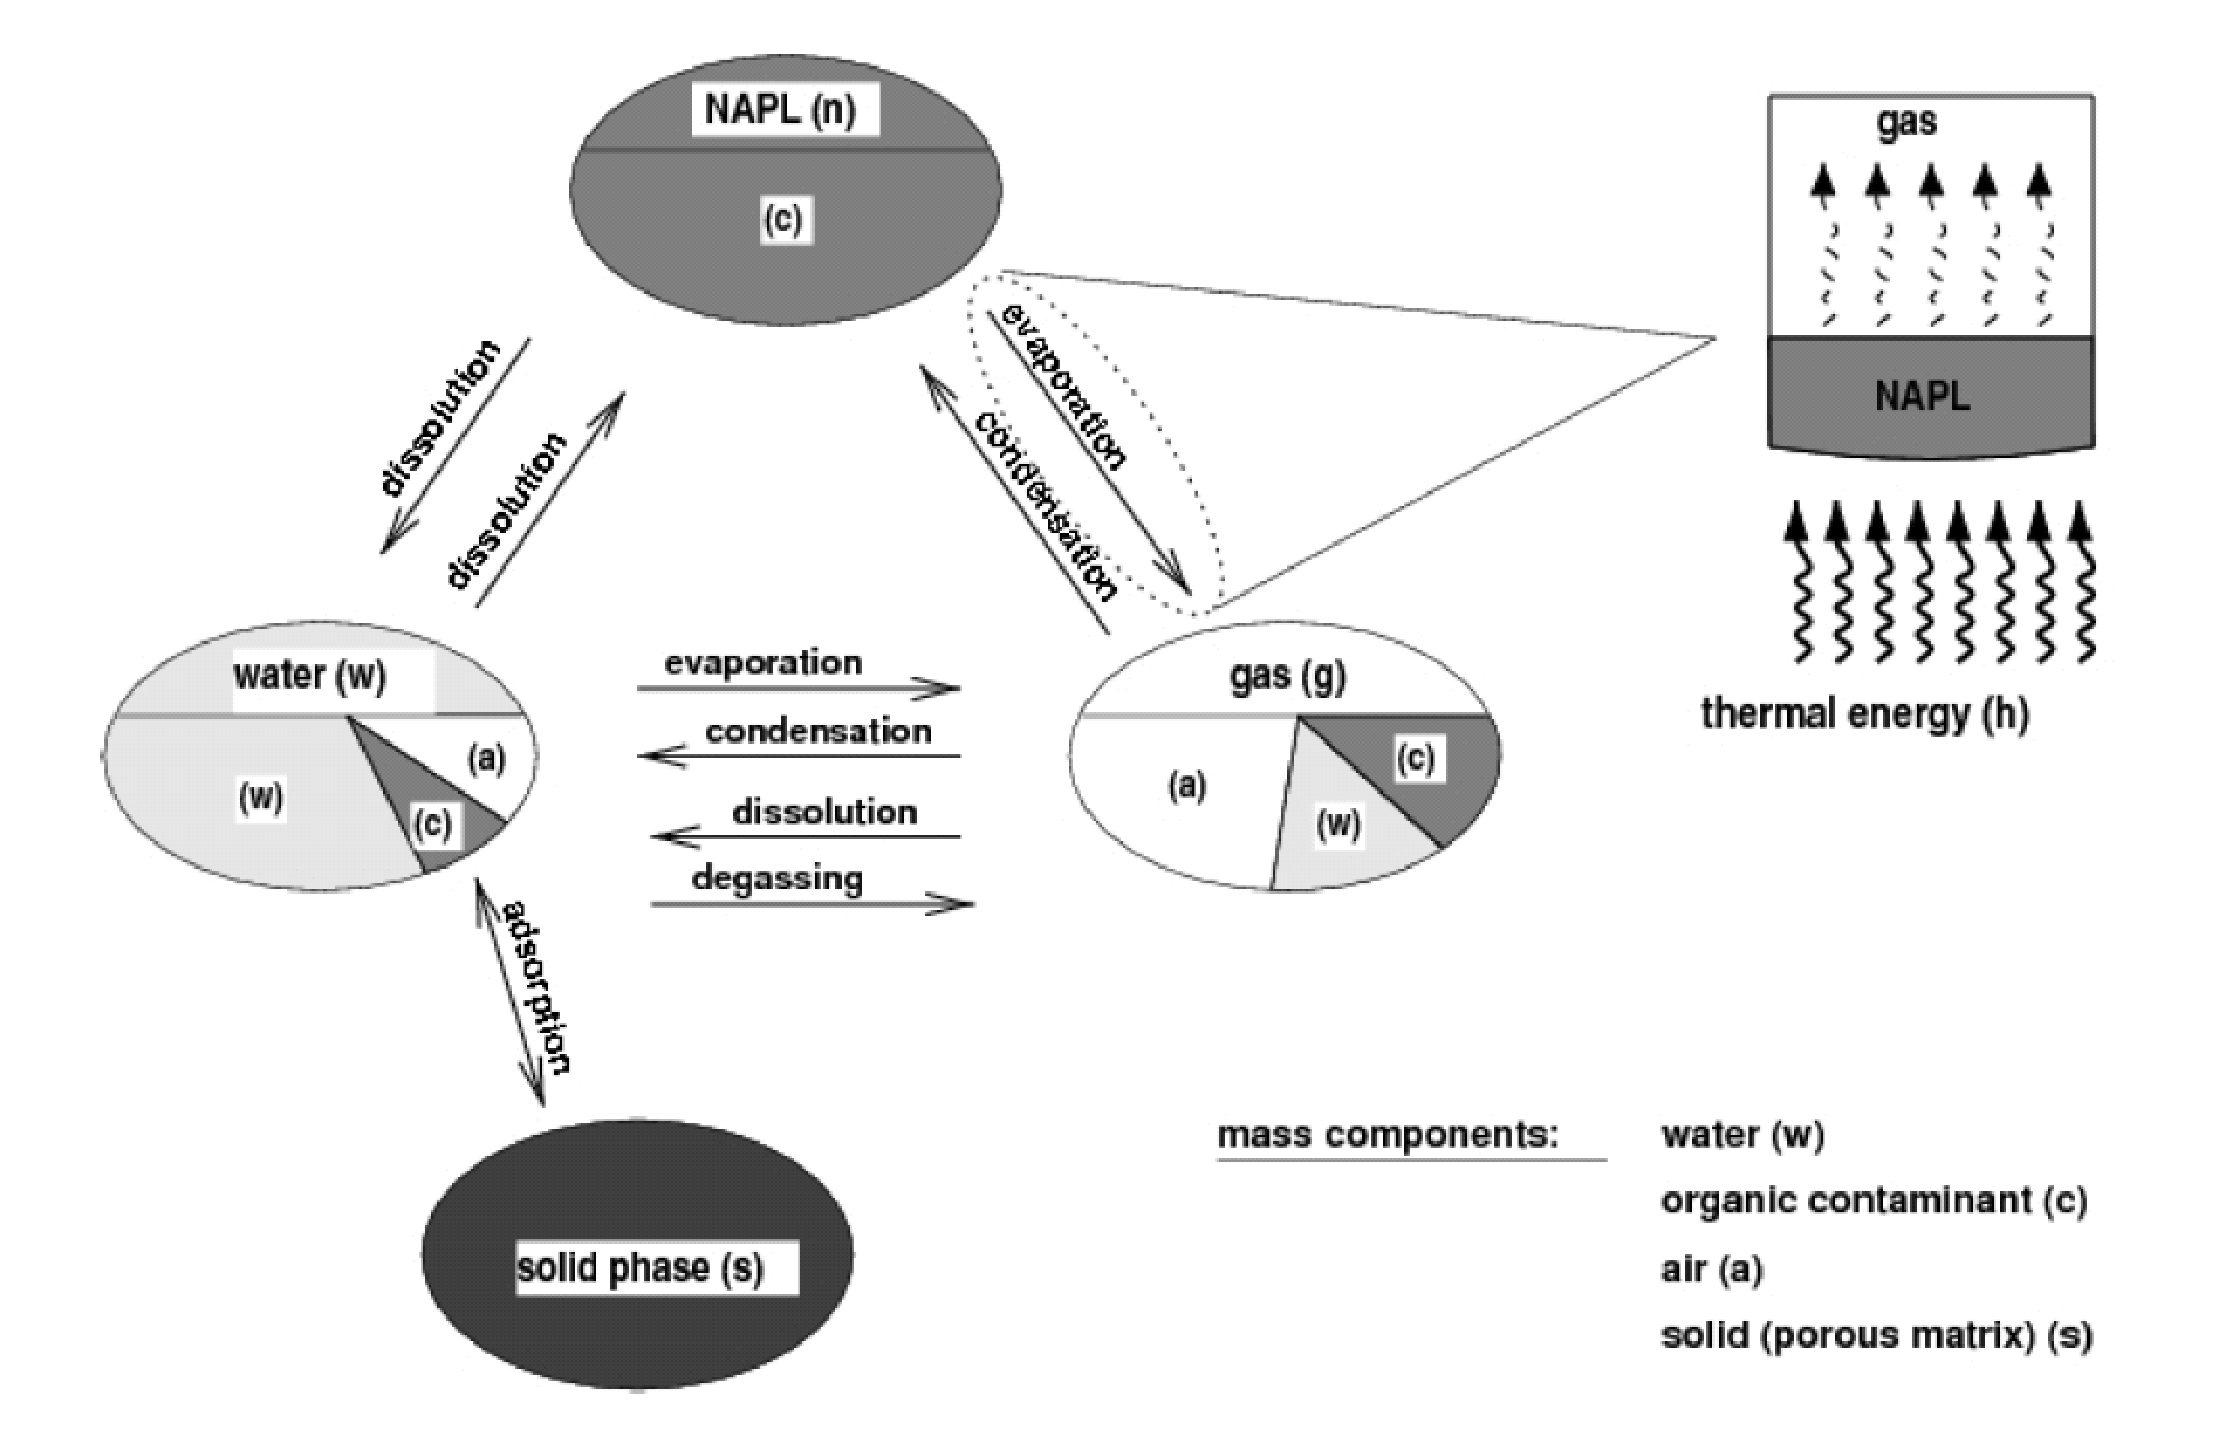
\includegraphics[width=0.7\linewidth]{EPS/masstransfer}
  \caption{Mass and energy transfer between the phases}
  \label{A3:fig:mundwtrans}
\end{figure}

\textbf{Equilibrium:}
For the nonisothermal multiphase processes in porous media under
consideration, we state that the assumption of local thermal
equilibrium is valid since flow velocities are small. We neglect
chemical reactions and biological decomposition and assume chemical
equilibrium.  Mechanical equilibrium is not valid in a porous medium, 
since discontinuities in pressure can occur across a fluid-fluid
interface due to capillary effects.

\textbf{Notation:} The index $\alpha \in \{\text{w}, \text{n}, \text{g}\}$ refers 
to the phase, while the superscript $\kappa \in \{\text{w}, \text{a}, \text{c}\}$ refers 
to the component. \\
\begin{tabular}{llll}
$p_\alpha$ & phase pressure & $\phi$ & porosity \\
$T$ & temperature & $K$ & absolute permeability tensor \\
$S_\alpha$ & phase saturation & $\tau$ & tortuosity \\
$x_\alpha^\kappa$ & mole fraction of component $\kappa$ in phase $\alpha$ & $\boldsymbol{g}$ & gravitational acceleration \\
$X_\alpha^\kappa$ & mass fraction of component $\kappa$ in phase $\alpha$ & $q^\kappa_\alpha$ & volume source term of $\kappa$ in $\alpha$ \\
$\varrho_{\text{mol},\alpha}$ & molar density of phase $\alpha$ & $u_\alpha$ & specific internal energy \\
$\varrho_{\alpha}$ & mass density of phase $\alpha$ & $h_\alpha$ & specific enthalpy \\
$k_{\text{r}\alpha}$ & relative permeability & $c_\text{s}$ & specific heat enthalpy \\
$\mu_\alpha$ & phase viscosity & $\lambda_\text{pm}$ & heat conductivity \\
$D_\alpha^\kappa$ & diffusivity of component $\kappa$ in phase $\alpha$ & $q^h$ & heat source term \\
$\boldsymbol{v}_\alpha$ & Darcy velocity & $\boldsymbol{v}_{a,\alpha}$  & advective velocity
\end{tabular}


\subsection{Balance Equations}
For the balance equations for multicomponent systems, it is in many
cases convenient to use a molar formulation of the continuity
equation. Considering the mass conservation for each component allows
us to drop source/sink terms for describing the mass transfer between
phases. Then, the
molar mass balance can be written as:
%
\begin{multline}
  \label{A3:eqmass1}
 \phi \frac{\partial (\sum_\alpha \varrho_{\text{mol}, \alpha}
    x_\alpha^\kappa S_\alpha )}{\partial t}  
 - \sum\limits_\alpha \Div \left( \frac{k_{\text{r}
        \alpha}}{\mu_\alpha} \varrho_{\text{mol}, \alpha}
    x_\alpha^\kappa K (\grad p_\alpha -
    \varrho_{\alpha} \boldsymbol{g}) \right)  \\
  % 
  %
 - \sum\limits_\alpha \Div \left( \tau \phi S_\alpha D_\alpha^\kappa \varrho_{\text{mol},
      \alpha} \grad x_\alpha^\kappa \right)  
 - q^\kappa = 0, \qquad \kappa \in \{\text{w,a,c}\}.
\end{multline}

The component mass balance can also be written in terms of mass fractions 
by replacing molar densities by mass densities and mole by mass fractions.
To obtain a single conserved quantity in the temporal derivative, the total 
concentration, representing the mass of one component per unit volume, is defined as
\begin{displaymath}
C^\kappa = \sum_\alpha \phi S_\alpha \varrho_{\text{mass},\alpha} X_\alpha^\kappa \; .
\end{displaymath}
Using this definition, the component mass balance is written as:

\begin{multline}
  \label{A3:eqmass2}
    \frac{\partial C^\kappa}{\partial t} = 
  \sum\limits_\alpha \Div \left( \frac{k_{\text{r}
        \alpha}}{\mu_\alpha} \varrho_{\text{mass}, \alpha}
    X_\alpha^\kappa K (\grad p_\alpha +
    \varrho_{\text{mass}, \alpha} \boldsymbol{g}) \right)  \\
  %
  %
   + \sum\limits_\alpha \Div \left( \tau \phi S_\alpha D_\alpha^\kappa \varrho_{\text{mass},
      \alpha} \grad X_\alpha^\kappa \right)  
 + q^\kappa = 0, \qquad \kappa \in \{\text{w,a,c}\}.
\end{multline}


In the case of non-isothermal systems, we further have to balance the
thermal energy. We assume fully reversible processes, such that entropy
is not needed as a model parameter. Furthermore, we neglect 
dissipative effects and the heat transport due to molecular
diffusion. The energy balance can then be
formulated as:
%
\begin{multline}
  \label{A3:eqenergmak1}
  \phi \frac{\partial \left( \sum_\alpha \varrho_{\alpha}
      u_\alpha S_\alpha \right)}{\partial t} + \left( 1 -
    \phi \right) \frac{\partial \varrho_{\text{s}} c_{\text{s}}
    T}{\partial t}  
 - \Div \left( \lambda_{\text{pm}} \grad T \right)
   \\
   - \sum\limits_\alpha \Div \left( \frac{k_{\text{r}
        \alpha}}{\mu_\alpha} \varrho_{\alpha} h_\alpha
    K \left( \grad p_\alpha - \varrho_{\alpha}
      \boldsymbol{g} \right) \right)  
 - q^h \; = \; 0.
\end{multline}

In order to close the system, supplementary constraints for capillary pressure, saturations and mole
fractions are needed, \cite{A3:helmig:1997}. 
According to the Gibbsian phase rule, the number of degrees of freedom
in a non-isothermal compositional multiphase system is equal to the
number of components plus one. This means we need as many independent
unknowns in the system description. The
available primary variables are, e.\ g., saturations, mole/mass
fractions, temperature, pressures, etc.

\section{Box method - A short introduction}\label{box}

For the spatial discretization the so called BOX-method is used which unites the advantages of the finite-volume (FV) and finite-element (FE) methods. 

First, the model domain $G$ is discretized with a FE mesh consisting of nodes i and corresponding elements $E_k$. Then, a secondary FV mesh is constructed by connecting the midpoints and barycenters of the elements surrounding node i creating a box $B_i$ around node i (see Figure \ref{pc:box}a). 

\begin{figure} [h]
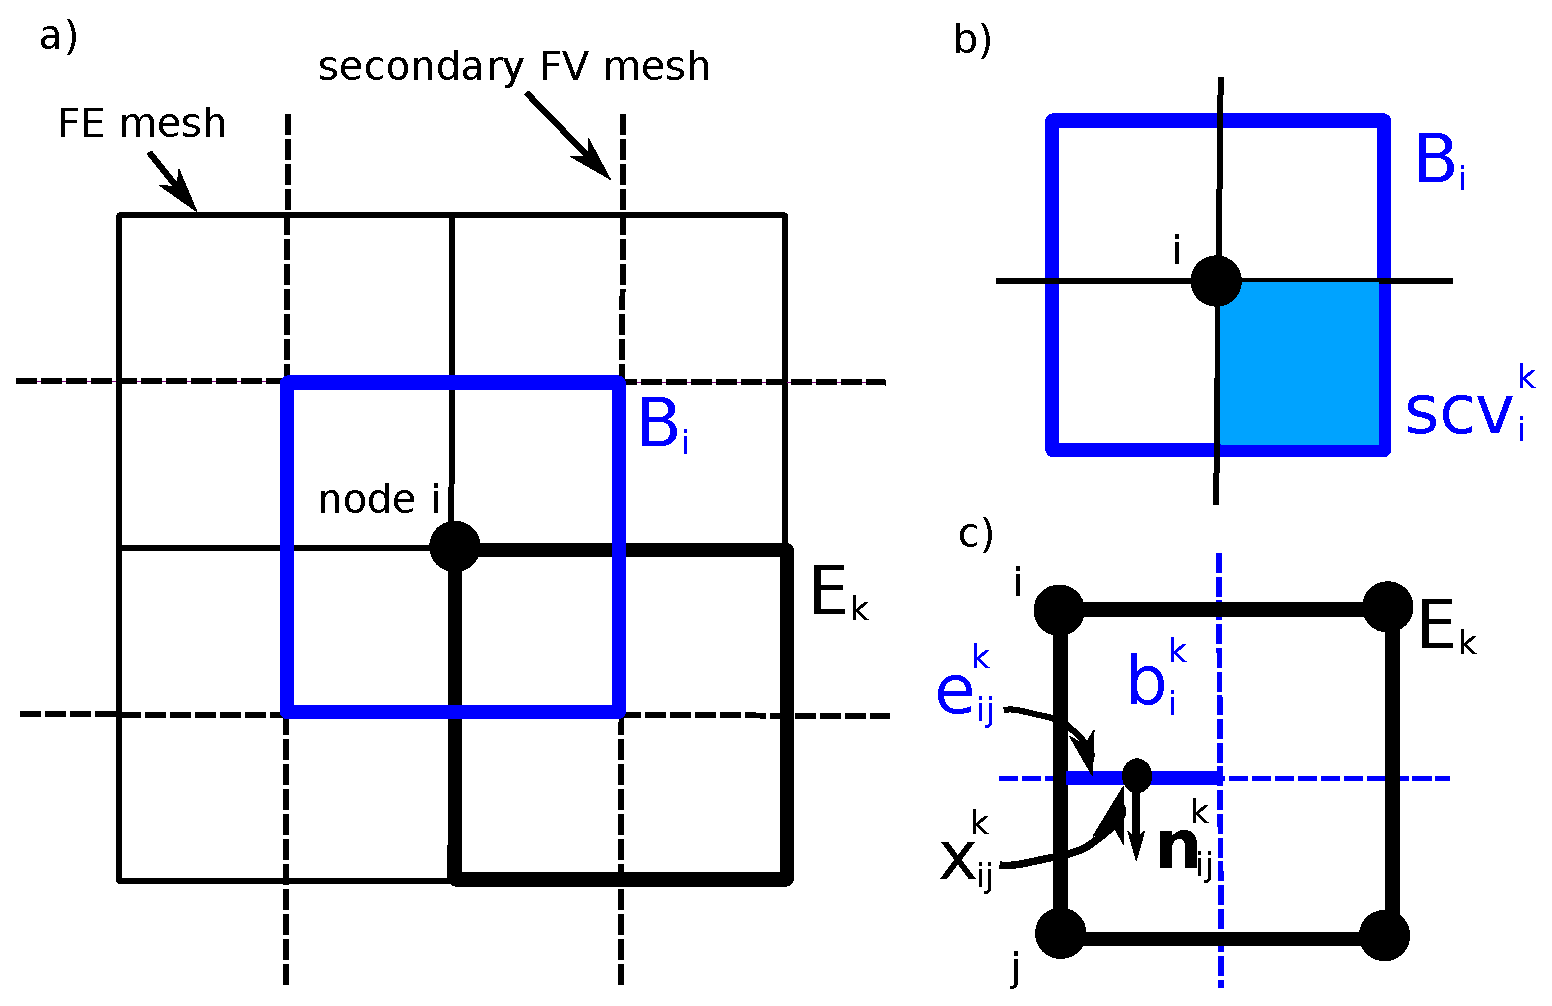
\includegraphics[width=0.8\linewidth,keepaspectratio]{EPS/box_disc}
\caption{\label{pc:box} Discretization of the BOX-method}
\end{figure}

The FE mesh divides the box $B_i$ into subcontrolvolumes (scv's) $b^k_i$ (see Figure \ref{pc:box}b). Figure \ref{pc:box}c shows the finite element $E_k$ and the scv's $b^k_i$ inside $E_k$, which belong to four different boxes $B_i$. Also necessary for the discretization are the faces of the subcontrolvolumes (scvf's) $e^k_{ij}$ between the scv's $b^k_i$ and $b^k_j$, where $|e^k_{ij}|$ is the length of the scvf. The integration points $x^k_{ij}$ on $e^k_{ij}$ and the outer normal vector $\mathbf n^k_{ij}$ are also to be defined (see Figure \ref{pc:box}c).

The advantage of the FE method is that unstructured grids can be used, while the FV method is mass conservative. The idea is to apply the FV method (balance of fluxes across the interfaces) to each FV box $B_i$  and to get the fluxes across the interfaces $e^k_{ij}$ at the integration points $x^k_{ij}$ from the FE approach. Consequently, at each scvf the following expression results:

\begin{equation}
 	f(\tilde u(x^k_{ij})) \cdot \mathbf n^k_{ij} \: |e^k_{ij}| \qquad \textrm{with} \qquad \tilde u(x^k_{ij}) = \sum_i N_i(x^k_{ij}) \cdot \hat u_i .
\end{equation}

In the following, the discretization of the balance equation is going to be derived. From the \textsc{Reynolds} transport theorem follows the general balance equation:

\begin{equation}
	\underbrace{\int_G \frac{\partial}{\partial t} \: u \: dG}_{1} + \underbrace{\int_{\partial G} (\mathbf{v} u + \mathbf w) \cdot \textbf n \: d\varGamma}_{2} = \underbrace{\int_G q \: dG}_{3}
\end{equation}

\begin{equation}
	f(u) = \int_G \frac{\partial u}{\partial t} \: dG + \int_{G} \nabla \cdot \underbrace{\left[  \mathbf{v} u + \mathbf w(u)\right] }_{F(u)}  \: dG - \int_G q \: dG = 0
\end{equation}
where term 1 describes the changes of entity $u$ within a control volume over time, term 2 the advective, diffusive and dispersive fluxes over the interfaces of the control volume and term 3 is the source and sink term. $G$ denotes the model domain and $F(u) = F(\mathbf v, p) = F(\mathbf v(x,t), p(x,t))$.

Like the FE method, the BOX-method follows the principle of weighted residuals. In the function $f(u)$ the unknown $u$ is approximated by discrete values at the nodes of the FE mesh $\hat u_i$ and linear basis functions $N_i$ yielding an approximate function $f(\tilde u)$. For $u\in \lbrace \mathbf v, p, x^\kappa \rbrace$ this means

\begin{minipage}[b]{0.47\textwidth}
\begin{equation}
\label{eq:p} 
	\tilde p = \sum_i N_i \hat{p_i}
\end{equation}
\begin{equation}
\label{eq:v} 
	\tilde{\mathbf v} = \sum_i N_i \hat{\mathbf v}
\end{equation}
\begin{equation}
\label{eq:x} 
	\tilde x^\kappa  = \sum_i N_i \hat x^\kappa 
\end{equation}
\end{minipage}
\hfill
\begin{minipage}[b]{0.47\textwidth}
\begin{equation}
\label{eq:dp} 
	\nabla \tilde p = \sum_i \nabla N_i \hat{p_i}
\end{equation}
\begin{equation}
\label{eq:dv} 
	\nabla \tilde{\mathbf v} = \sum_i \nabla N_i \hat{\mathbf v}
\end{equation}
\begin{equation}
\label{eq:dx} 
	\nabla \tilde x^\kappa  = \sum_i \nabla N_i \hat x^\kappa .
\end{equation}
\end{minipage} 

Due to the approximation with node values and basis functions the differential equations are not exactly fulfilled anymore but a residual $\varepsilon$ is produced.

\begin{equation}
	f(u) = 0  \qquad \Rightarrow \qquad f(\tilde u) = \varepsilon
\end{equation}

Application of the principle of weighted residuals, meaning the multiplication of the residual $\varepsilon$ with a weighting function $W_j$  and claiming that this product has to vanish within the whole domain,

\begin{equation}
	\int_G W_j \cdot \varepsilon \: \overset {!}{=} \: 0 \qquad \textrm{with} \qquad \sum_j W_j =1
\end{equation}
yields the following equation:

\begin{equation}
	\int_G W_j \frac{\partial \tilde u}{\partial t} \: dG + \int_G W_j \cdot \left[ \nabla \cdot F(\tilde u) \right]  \: dG - \int_G W_j \cdot q \: dG = \int_G W_j \cdot \varepsilon \: dG \: \overset {!}{=} \: 0 .
\end{equation}

Then, the chain rule and the \textsc{Green-Gaussian} integral theorem are applied.

\begin{equation}
	\int_G W_j \frac{\partial \sum_i N_i \hat u_i}{\partial t} \: dG + \int_{\partial G}  \left[ W_j \cdot F(\tilde u)\right]  \cdot \mathbf n \: d\varGamma_G + \int_G  \nabla W_j \cdot F(\tilde u)  \: dG - \int_G W_j \cdot q \: dG = 0
\end{equation}

A mass lumping technique is applied by assuming that the storage capacity is reduced to the nodes. This means that the integrals $M_{i,j} = \int_G W_j \: N_i \: dG$ are replaced by the mass lumping term $M^{lump}_{i,j}$ which is defined as:

\begin{equation}
	 M^{lump}_{i,j} =\begin{cases} \int_G W_j \: dG = \int_G N_i \: dG = V_i &i = j\\
	0 &i \neq j\\
	         \end{cases}
\end{equation}
where $V_i$ is the volume of the FV box $B_i$ associated with node i. The application of this assumption in combination with $\int_G W_j \:q \: dG = V_i \: q$ yields

\begin{equation}
	V_i \frac{\partial \hat u_i}{\partial t} + \int_{\partial G}  \left[ W_j \cdot F(\tilde u)\right]  \cdot \mathbf n \: d\varGamma_G + \int_G  \nabla W_j \cdot F(\tilde u)  \: dG- V_i \cdot q = 0 \, .
\end{equation}

Defining the weighting function $W_j$ to be piecewisely constant over a control volume box $B_i$ 

\begin{equation}
	W_j(x) = \begin{cases}
	          1 &x \in B_i \\
		  0 &x \notin B_i\\
	         \end{cases}
\end{equation}

causes $\nabla W_j = 0$:

\begin{equation}
\label{eq:disc1} 
	V_i \frac{\partial \hat u_i}{\partial t} + \int_{\partial B_i}  \left[ W_j \cdot F(\tilde u)\right] \cdot \mathbf n  \;  d{\varGamma}_{B_i} - V_i \cdot q = 0 .
\end{equation}

The consideration of the time discretization and inserting $W_j = 1$ finally lead to the discretized form which will be applied to the mathematical flow and transport equations:

\begin{equation}
\label{eq:discfin} 
	V_i \frac{\hat u_i^{n+1} - \hat u_i^{n}}{\Delta t} + \int_{\partial B_i}  F(\tilde u^{n+1}) \cdot \mathbf n  \;  d{\varGamma}_{B_i} - V_i \: q^{n+1} \: = 0 
\end{equation}



\section{Available models} 
The following description of the available models is automatically extracted 
from the Doxygen documentation.
% \textbf{TODO}: Unify notation. 

\subsection{Fully-implicit models} 

The fully-implicit models described in this section are using the box
scheme as described in Section \ref{box} for spatial and the implicit Euler
method as temporal discretization. The models themselves are located in
subdirectories of \texttt{dumux/boxmodels} of the \Dumux distribution.

\subsubsection{The single-phase model: OnePBoxModel} 
Single phase isothermal flow model is implemented for compressible flow. \begin{align*} \phi \frac{\partial \varrho}{\partial t} + \vec{\nabla} \cdot (- \varrho \frac{\bar{\bar{K}}}{\mu} ( \nabla p -\varrho \vec{g})) = q \end{align*} However, the model can also be used for incompressible single pahse flow modeling, when in problem file a fluid with constant density is chosen. 


\subsubsection{The single-phase, two-component model:  OnePTwoCBoxModel} 
%%%%%%%%%%%%%%%%%%%%%%%%%%%%%%%%%%%%%%%%%%%%%%%%%%%%%%%%%%%%%%%%%
% This file has been autogenerated from the LaTeX part of the   %
% doxygen documentation; DO NOT EDIT IT! Change the model's .hh %
% file instead!!                                                %
%%%%%%%%%%%%%%%%%%%%%%%%%%%%%%%%%%%%%%%%%%%%%%%%%%%%%%%%%%%%%%%%%

\-This model implements a one-\/phase flow of a compressible fluid, that consists of two components, using a standard \-Darcy approach as the equation for the conservation of momentum\-: \[ v_{D} = - \frac{\textbf K}{\mu} \left(\text{grad} p - \varrho {\textbf g} \right) \]

\-Gravity can be enabled or disabled via the property system. \-By inserting this into the continuity equation, one gets \[ \Phi \frac{\partial \varrho}{\partial t} - \text{div} \left\{ \varrho \frac{\textbf K}{\mu} \left(\text{grad}\, p - \varrho {\textbf g} \right) \right\} = q \;, \]

\-The transport of the components is described by the following equation\-: \[ \Phi \frac{ \partial \varrho x}{\partial t} - \text{div} \left( \varrho \frac{{\textbf K} x}{\mu} \left( \text{grad}\, p - \varrho {\textbf g} \right) + \varrho \tau \Phi D \text{grad} x \right) = q. \]

\-All equations are discretized using a fully-\/coupled vertex-\/centered finite volume (box) scheme as spatial and the implicit \-Euler method as time discretization.

\-The primary variables are the pressure $p$ and the mole or mass fraction of dissolved component $x$.



\subsubsection{The two-phase model using the Richards assumption: RichardsBoxModel} 
%%%%%%%%%%%%%%%%%%%%%%%%%%%%%%%%%%%%%%%%%%%%%%%%%%%%%%%%%%%%%%%%%
% This file has been autogenerated from the LaTeX part of the   %
% doxygen documentation; DO NOT EDIT IT! Change the model's .hh %
% file instead!!                                                %
%%%%%%%%%%%%%%%%%%%%%%%%%%%%%%%%%%%%%%%%%%%%%%%%%%%%%%%%%%%%%%%%%


This model implements a variant of the Richards equation for quasi-\/twophase flow. In the unsaturated zone, Richards' equation is frequently used to calculate the water distribution above the groundwater level. It can be derived from the twophase equations, i.e. \[ \frac{\partial\;\phi S_\alpha \rho_\alpha}{\partial t} - \mathbf{div} \left\{ \rho_\alpha \frac{k_{r\alpha}}{\mu_\alpha}\;K \mathbf{grad}\left[ p_\alpha - g\rho_\alpha \right] \right\} = q_\alpha, \] where $\alpha \in \{w, n\}$ is the fluid phase, $\rho_\alpha$ is the fluid density, $S_\alpha$ is the fluid saturation, $\phi$ is the porosity of the soil, $k_{r\alpha}$ is the relative permeability for the fluid, $\mu_\alpha$ is the fluid's dynamic viscosity, $K$ is the intrinsic permeability, $p_\alpha$ is the fluid pressure and $g$ is the potential of the gravity field.

In contrast to the full twophase model, the Richards model assumes gas as the non-\/wetting fluid and that it exhibits a much lower viscosity than the (liquid) wetting phase. (For example at atmospheric pressure and at room temperature, the viscosity of air is only about $1\%$ of the viscosity of liquid water.) As a consequence, the $\frac{k_{r\alpha}}{\mu_\alpha}$ term typically is much larger for the gas phase than for the wetting phase. For this reason, the Richards model assumes that $\frac{k_{rn}}{\mu_n}$ tends to infinity. This implies that the pressure of the gas phase is equivalent to a static pressure and can thus be specified externally and that therefore, mass conservation only needs to be considered for the wetting phase.

The model thus choses the absolute pressure of the wetting phase $p_w$ as its only primary variable. The wetting phase saturation is calculated using the inverse of the capillary pressure, i.e. \[ S_w = p_c^{-1}(p_n - p_w) \] holds, where $p_n$ is a given reference pressure. Nota bene that the last step is assumes that the capillary pressure-\/saturation curve can be inverted uniquely, so it is not possible to set the capillary pressure to zero when using the Richards model!



\subsubsection{The two-phase model: TwoPBoxModel}
This model implements two-phase flow of two completely immiscible fluids $\alpha \in \{ w, n \}$ using a standard multiphase Darcy approach as the equation for the conservation of momentum: \[ \vec{v_\alpha} = - \frac{k_{r\alpha}}{\mu_\alpha} K \left(\grad p_\alpha - \varrho_{\alpha} \boldsymbol{g} \right) \]

By inserting this into the equation for the conservation of the phase mass, one gets \[ \phi \frac{\partial \varrho_\alpha S_\alpha}{\partial t} - \Div \left\{ \varrho_\alpha \frac{k_{r\alpha}}{\mu_\alpha} K \left(\grad p_\alpha - \varrho_{\alpha} \boldsymbol{g} \right) \right\} = q_\alpha \;, \] which is discretized by this model using the fully-coupled vertex centered finite volume (box) scheme as spatial and the implicit Euler method as time discretization.

By using constitutive relations for the capillary pressure $p_c = p_n - p_w$ and relative permability $k_{r\alpha}$ and taking advantage of the fact that $S_w + S_n = 1$, the number of unknowns can be reduced to two. Currently the model supports chosing either $p_w$ and $S_n$ or $p_n$ and $S_w$ as primary variables. The formulation which ought to be used can be specified by setting the {\tt Formulation} property to either either {\tt \doxyref{TwoPIndices::pWsN}{p.}{structDune_1_1TwoPIndices_7bab78f10df58319eafe8b79a1d28553}} or {\tt \doxyref{TwoPIndices::pNsW}{p.}{structDune_1_1TwoPIndices_b2b28761c782605cf080f9b6f9b618b5}}. By default, the model uses $p_w$ and $S_n$. 


\subsubsection{The non-isothermal two-phase model: TwoPNIBoxModel} 
This model implements a non-isothermal two-phase flow of two completely immiscible fluids $\alpha \in \{ w, n \}$. Using the standard multiphase Darcy approach the mass conservation equations for both phases can be described as follows: \begin{eqnarray*} && \phi \frac{\partial (\sum_\alpha \varrho_\alpha S_\alpha )}{\partial t} - \sum_\alpha \Div \left\{ \varrho_\alpha \frac{k_{r\alpha}}{\mu_\alpha} \mbox{\bf K} (\grad p_\alpha - \varrho_{\alpha} \mbox{\bf g}) \right\} - \sum_\alpha q_\alpha^\kappa = \quad 0 \qquad \alpha \in \{w, n\} \end{eqnarray*} For the energy balance local thermal equilibrium is assumed which results in one energy conservation equation for the porous solid matrix and the fluids: \begin{eqnarray*} && \phi \frac{\partial \left( \sum_\alpha \varrho_\alpha u_\alpha S_\alpha \right)}{\partial t} + \left( 1 - \phi \right) \frac{\partial (\varrho_s c_s T)}{\partial t} - \sum_\alpha \Div \left\{ \varrho_\alpha h_\alpha \frac{k_{r\alpha}}{\mu_\alpha} \mathbf{K} \left( \grad \: p_\alpha - \varrho_\alpha \mathbf{g} \right) \right\} \\ &-& \Div \left( \lambda_{pm} \grad \: T \right) - q^h \qquad = \quad 0 \qquad \alpha \in \{w, n\} \end{eqnarray*}

the equations are discretized by this model using the fully-coupled vertex centered finite volume (box) scheme as spatial and the implicit Euler method as time discretization.

Currently the model supports chosing either $p_w$, $S_n$ and $T$ or $p_n$, $S_w$ and $T$ as primary variables. The formulation which ought to be used can be specified by setting the {\tt Formulation} property to either either {\tt \doxyref{TwoPNIIndices::pWsN}{p.}{structDune_1_1TwoPIndices_7bab78f10df58319eafe8b79a1d28553}} or {\tt \doxyref{TwoPIndices::pNsW}{p.}{structDune_1_1TwoPIndices_b2b28761c782605cf080f9b6f9b618b5}}. By default, the model uses $p_w$, $S_n$ and $T$. 


\subsubsection{The two-phase, two-component model: TwoPTwoCBoxModel} 
%%%%%%%%%%%%%%%%%%%%%%%%%%%%%%%%%%%%%%%%%%%%%%%%%%%%%%%%%%%%%%%%%
% This file has been autogenerated from the LaTeX part of the   %
% doxygen documentation; DO NOT EDIT IT! Change the model's .hh %
% file instead!!                                                %
%%%%%%%%%%%%%%%%%%%%%%%%%%%%%%%%%%%%%%%%%%%%%%%%%%%%%%%%%%%%%%%%%


Adaption of the BOX scheme to the two-\/phase two-\/component flow model. This model implements two-\/phase two-\/component flow of two compressible and partially miscible fluids $\alpha \in \{ w, n \}$ composed of the two components $\kappa \in \{ w, a \}$. The standard multiphase Darcy approach is used as the equation for the conservation of momentum: \[ v_\alpha = - \frac{k_{r\alpha}}{\mu_\alpha} \mbox{\bf K} \left(\text{grad}\, p_\alpha - \varrho_{\alpha} \mbox{\bf g} \right) \]

By inserting this into the equations for the conservation of the components, one gets one transport equation for each component \begin{eqnarray} && \phi \frac{\partial (\sum_\alpha \varrho_\alpha X_\alpha^\kappa S_\alpha )} {\partial t} - \sum_\alpha \text{div} \left\{ \varrho_\alpha X_\alpha^\kappa \frac{k_{r\alpha}}{\mu_\alpha} \mbox{\bf K} (\text{grad}\, p_\alpha - \varrho_{\alpha} \mbox{\bf g}) \right\} \nonumber \\ \nonumber \\ &-& \sum_\alpha \text{div} \left\{{\bf D_{\alpha, pm}^\kappa} \varrho_{\alpha} \text{grad}\, X^\kappa_{\alpha} \right\} - \sum_\alpha q_\alpha^\kappa = 0 \qquad \kappa \in \{w, a\} \, , \alpha \in \{w, g\} \end{eqnarray}

This is discretized using a fully-\/coupled vertex centered finite volume (box) scheme as spatial and the implicit Euler method as temporal discretization.

By using constitutive relations for the capillary pressure $p_c = p_n - p_w$ and relative permeability $k_{r\alpha}$ and taking advantage of the fact that $S_w + S_n = 1$ and $X^\kappa_w + X^\kappa_n = 1$, the number of unknowns can be reduced to two. The used primary variables are, like in the two-\/phase model, either $p_w$ and $S_n$ or $p_n$ and $S_w$. The formulation which ought to be used can be specified by setting the {\ttfamily Formulation} property to either TwoPTwoCIndices::pWsN or TwoPTwoCIndices::pNsW. By default, the model uses $p_w$ and $S_n$. Moreover, the second primary variable depends on the phase state, since a primary variable switch is included. The phase state is stored for all nodes of the system. Following cases can be distinguished:
\begin{itemize}
\item Both phases are present: The saturation is used (either $S_n$ or $S_w$, dependent on the chosen {\ttfamily Formulation}), as long as $ 0 < S_\alpha < 1$.
\item Only wetting phase is present: The mass fraction of, e.g., air in the wetting phase $X^a_w$ is used, as long as the maximum mass fraction is not exceeded ( $X^a_w<X^a_{w,max}$)
\item Only non-\/wetting phase is present: The mass fraction of, e.g., water in the non-\/wetting phase, $X^w_n$, is used, as long as the maximum mass fraction is not exceeded ( $X^w_n<X^w_{n,max}$)
\end{itemize}



\subsubsection{The non-isothermal two-phase, two-component model: TwoPTwoCNIBoxModel} 
%%%%%%%%%%%%%%%%%%%%%%%%%%%%%%%%%%%%%%%%%%%%%%%%%%%%%%%%%%%%%%%%%
% This file has been autogenerated from the LaTeX part of the   %
% doxygen documentation; DO NOT EDIT IT! Change the model's .hh %
% file instead!!                                                %
%%%%%%%%%%%%%%%%%%%%%%%%%%%%%%%%%%%%%%%%%%%%%%%%%%%%%%%%%%%%%%%%%

\-This model implements a non-\/isothermal two-\/phase flow of two compressible and partly miscible fluids $\alpha \in \{ w, n \}$. \-Thus each component $\kappa \{ w, a \}$ can be present in each phase. \-Using the standard multiphase \-Darcy approach a mass balance equation is solved\-: \begin{eqnarray*} && \phi \frac{\partial (\sum_\alpha \varrho_\alpha X_\alpha^\kappa S_\alpha )}{\partial t} - \sum_\alpha \text{div} \left\{ \varrho_\alpha X_\alpha^\kappa \frac{k_{r\alpha}}{\mu_\alpha} \mbox{\bf K} (\text{grad}\, p_\alpha - \varrho_{\alpha} \mbox{\bf g}) \right\}\\ &-& \sum_\alpha \text{div} \left\{{\bf D}_{\alpha, pm}^\kappa \varrho_{\alpha} \text{grad}\, X^\kappa_{\alpha} \right\} - \sum_\alpha q_\alpha^\kappa = 0 \qquad \kappa \in \{w, a\} \, , \alpha \in \{w, n\} \end{eqnarray*} \-For the energy balance, local thermal equilibrium is assumed which results in one energy conservation equation for the porous solid matrix and the fluids\-: \begin{eqnarray*} && \phi \frac{\partial \left( \sum_\alpha \varrho_\alpha u_\alpha S_\alpha \right)}{\partial t} + \left( 1 - \phi \right) \frac{\partial (\varrho_s c_s T)}{\partial t} - \sum_\alpha \text{div} \left\{ \varrho_\alpha h_\alpha \frac{k_{r\alpha}}{\mu_\alpha} \mathbf{K} \left( \text{grad}\, p_\alpha - \varrho_\alpha \mathbf{g} \right) \right\} \\ &-& \text{div} \left( \lambda_{pm} \text{grad} \, T \right) - q^h = 0 \qquad \alpha \in \{w, n\} \end{eqnarray*}

\-This is discretized using a fully-\/coupled vertex centered finite volume (box) scheme as spatial and the implicit \-Euler method as temporal discretization.

\-By using constitutive relations for the capillary pressure $p_c = p_n - p_w$ and relative permeability $k_{r\alpha}$ and taking advantage of the fact that $S_w + S_n = 1$ and $X^\kappa_w + X^\kappa_n = 1$, the number of unknowns can be reduced to two. \-If both phases are present the primary variables are, like in the nonisothermal two-\/phase model, either $p_w$, $S_n$ and temperature or $p_n$, $S_w$ and temperature. \-The formulation which ought to be used can be specified by setting the {\ttfamily \-Formulation} property to either {\ttfamily \-Two\-P\-Two\-Indices\-::p\-Ws\-N} or {\ttfamily \-Two\-P\-Two\-C\-Indices\-::p\-Ns\-W}. \-By default, the model uses $p_w$ and $S_n$. \-In case that only one phase (nonwetting or wetting phase) is present the second primary variable represents a mass fraction. \-The correct assignment of the second primary variable is performed by a phase state dependent primary variable switch. \-The phase state is stored for all nodes of the system. \-The following cases can be distinguished\-:
\begin{itemize}
\item \-Both phases are present\-: \-The saturation is used (either $S_n$ or $S_w$, dependent on the chosen formulation).
\item \-Only wetting phase is present\-: \-The mass fraction of air in the wetting phase $X^a_w$ is used.
\item \-Only non-\/wetting phase is present\-: \-The mass fraction of water in the non-\/wetting phase, $X^w_n$, is used.
\end{itemize}



\subsubsection{The three-phase, three-component model: ThreePThreeCBoxModel}
%%%%%%%%%%%%%%%%%%%%%%%%%%%%%%%%%%%%%%%%%%%%%%%%%%%%%%%%%%%%%%%%%
% This file has been autogenerated from the LaTeX part of the   %
% doxygen documentation; DO NOT EDIT IT! Change the model's .hh %
% file instead!!                                                %
%%%%%%%%%%%%%%%%%%%%%%%%%%%%%%%%%%%%%%%%%%%%%%%%%%%%%%%%%%%%%%%%%

\-This model implements three-\/phase three-\/component flow of three fluid phases $\alpha \in \{ water, gas, NAPL \}$ each composed of up to three components $\kappa \in \{ water, air, contaminant \}$. \-The standard multiphase \-Darcy approach is used as the equation for the conservation of momentum\-: \[ v_\alpha = - \frac{k_{r\alpha}}{\mu_\alpha} \mbox{\bf K} \left(\text{grad}\, p_\alpha - \varrho_{\alpha} \mbox{\bf g} \right) \]

\-By inserting this into the equations for the conservation of the components, one transport equation for each component is obtained as \begin{eqnarray} && \phi \frac{\partial (\sum_\alpha \varrho_{\text{mol}, \alpha} x_\alpha^\kappa S_\alpha )}{\partial t} - \sum\limits_\alpha \text{div} \left\{ \frac{k_{r\alpha}}{\mu_\alpha} \varrho_{\text{mol}, \alpha} x_\alpha^\kappa \mbox{\bf K} (\text{grad}\, p_\alpha - \varrho_{\text{mass}, \alpha} \mbox{\bf g}) \right\} \nonumber \\ \nonumber \\ && - \sum\limits_\alpha \text{div} \left\{ D_{pm}^\kappa \varrho_{\text{mol}, \alpha } \text{grad}\, x_\alpha^\kappa \right\} - q^\kappa = 0 \qquad \forall \kappa , \; \forall \alpha \end{eqnarray}

\-Note that these balance equations are molar.

\-The equations are discretized using a fully-\/coupled vertex centered finite volume (\-B\-O\-X) scheme as spatial scheme and the implicit \-Euler method as temporal discretization.

\-The model uses commonly applied auxiliary conditions like $S_w + S_n + S_g = 1$ for the saturations and $x^w_\alpha + x^a_\alpha + x^c_\alpha = 1$ for the mole fractions. \-Furthermore, the phase pressures are related to each other via capillary pressures between the fluid phases, which are functions of the saturation, e.\-g. according to the approach of \-Parker et al.

\-The used primary variables are dependent on the locally present fluid phases \-An adaptive primary variable switch is included. \-The phase state is stored for all nodes of the system. \-The following cases can be distinguished\-:
\begin{itemize}
\item \-All three phases are present\-: \-Primary variables are two saturations ( $S_w$ and $S_n$, and a pressure, in this case $p_g$.
\item \-Only the water phase is present\-: \-Primary variables are now the mole fractions of air and contaminant in the water phase ( $x_w^a$ and $x_w^c$), as well as the gas pressure, which is, of course, in a case where only the water phase is present, just the same as the water pressure.
\item \-Gas and \-N\-A\-P\-L phases are present\-: \-Primary variables ( $S_n$, $x_g^w$, $p_g$).
\item \-Water and \-N\-A\-P\-L phases are present\-: \-Primary variables ( $S_n$, $x_w^a$, $p_g$).
\item \-Only gas phase is present\-: \-Primary variables ( $x_g^w$, $x_g^c$, $p_g$).
\item \-Water and gas phases are present\-: \-Primary variables ( $S_w$, $x_w^g$, $p_g$).
\end{itemize}



\subsubsection{The non-isothermal three-phase, three-component model: ThreePThreeCNIBoxModel} 
%%%%%%%%%%%%%%%%%%%%%%%%%%%%%%%%%%%%%%%%%%%%%%%%%%%%%%%%%%%%%%%%%
% This file has been autogenerated from the LaTeX part of the   %
% doxygen documentation; DO NOT EDIT IT! Change the model's .hh %
% file instead!!                                                %
%%%%%%%%%%%%%%%%%%%%%%%%%%%%%%%%%%%%%%%%%%%%%%%%%%%%%%%%%%%%%%%%%

\-This model implements three-\/phase three-\/component flow of three fluid phases $\alpha \in \{ water, gas, NAPL \}$ each composed of up to three components $\kappa \in \{ water, air, contaminant \}$. \-The standard multiphase \-Darcy approach is used as the equation for the conservation of momentum\-: \[ v_\alpha = - \frac{k_{r\alpha}}{\mu_\alpha} \mbox{\bf K} \left(\text{grad}\, p_\alpha - \varrho_{\alpha} \mbox{\bf g} \right) \]

\-By inserting this into the equations for the conservation of the components, one transport equation for each component is obtained as \begin{eqnarray*} && \phi \frac{\partial (\sum_\alpha \varrho_{\text{mol}, \alpha} x_\alpha^\kappa S_\alpha )}{\partial t} - \sum\limits_\alpha \text{div} \left\{ \frac{k_{r\alpha}}{\mu_\alpha} \varrho_{\text{mol}, \alpha} x_\alpha^\kappa \mbox{\bf K} (\text{grad}\; p_\alpha - \varrho_{\text{mass}, \alpha} \mbox{\bf g}) \right\} \nonumber \\ \nonumber \\ && - \sum\limits_\alpha \text{div} \left\{ D_{pm}^\kappa \varrho_{\text{mol}, \alpha } \text{grad} \; x_\alpha^\kappa \right\} - q^\kappa = 0 \qquad \forall \kappa , \; \forall \alpha \end{eqnarray*}

\-Note that these balance equations above are molar. \-In addition to that, a single balance of thermal energy is formulated for the fluid-\/filled porous medium under the assumption of local thermal equilibrium \begin{eqnarray*} && \phi \frac{\partial \left( \sum_\alpha \varrho_\alpha u_\alpha S_\alpha \right)}{\partial t} + \left( 1 - \phi \right) \frac{\partial (\varrho_s c_s T)}{\partial t} - \sum_\alpha \text{div} \left\{ \varrho_\alpha h_\alpha \frac{k_{r\alpha}}{\mu_\alpha} \mathbf{K} \left( \text{grad}\, p_\alpha - \varrho_\alpha \mathbf{g} \right) \right\} \\ &-& \text{div} \left( \lambda_{pm} \text{grad} \, T \right) - q^h = 0 \qquad \alpha \in \{w, n, g\} \end{eqnarray*}

\-The equations are discretized using a fully-\/coupled vertex centered finite volume (\-B\-O\-X) scheme as spatial scheme and the implicit \-Euler method as temporal discretization.

\-The model uses commonly applied auxiliary conditions like $S_w + S_n + S_g = 1$ for the saturations and $x^w_\alpha + x^a_\alpha + x^c_\alpha = 1$ for the mole fractions. \-Furthermore, the phase pressures are related to each other via capillary pressures between the fluid phases, which are functions of the saturation, e.\-g. according to the approach of \-Parker et al.

\-The used primary variables are dependent on the locally present fluid phases \-An adaptive primary variable switch is included. \-The phase state is stored for all nodes of the system. \-The following cases can be distinguished\-:
\begin{itemize}
\item \-All three phases are present\-: \-Primary variables are two saturations ( $S_w$ and $S_n$, a pressure, in this case $p_g$, and the temperature $T$.
\item \-Only the water phase is present\-: \-Primary variables are now the mole fractions of air and contaminant in the water phase ( $x_w^a$ and $x_w^c$), as well as temperature and the gas pressure, which is, of course, in a case where only the water phase is present, just the same as the water pressure.
\item \-Gas and \-N\-A\-P\-L phases are present\-: \-Primary variables ( $S_n$, $x_g^w$, $p_g$, $T$).
\item \-Water and \-N\-A\-P\-L phases are present\-: \-Primary variables ( $S_n$, $x_w^a$, $p_g$, $T$).
\item \-Only gas phase is present\-: \-Primary variables ( $x_g^w$, $x_g^c$, $p_g$, $T$).
\item \-Water and gas phases are present\-: \-Primary variables ( $S_w$, $x_w^g$, $p_g$, $T$).
\end{itemize}



\subsubsection{The $M$-phase, $N$-component model: MpNcBoxModel} 
%%%%%%%%%%%%%%%%%%%%%%%%%%%%%%%%%%%%%%%%%%%%%%%%%%%%%%%%%%%%%%%%%
% This file has been autogenerated from the LaTeX part of the   %
% doxygen documentation; DO NOT EDIT IT! Change the model's .hh %
% file instead!!                                                %
%%%%%%%%%%%%%%%%%%%%%%%%%%%%%%%%%%%%%%%%%%%%%%%%%%%%%%%%%%%%%%%%%

\-This model implements a $M$-\/phase flow of a fluid mixture composed of $N$ chemical species. \-The phases are denoted by lower index $\alpha \in \{ 1, \dots, M \}$. \-All fluid phases are mixtures of $N \geq M - 1$ chemical species which are denoted by the upper index $\kappa \in \{ 1, \dots, N \} $.

\-The standard multi-\/phase \-Darcy law is used as the equation for the conservation of momentum\-: \[ v_\alpha = - \frac{k_{r\alpha}}{\mu_\alpha} \boldsymbol{K} \left( \text{grad}\left(p_\alpha - \varrho_{\alpha} g\right) \right) \]

\-By inserting this into the equations for the conservation of the mass of each component, one gets one mass-\/continuity equation for each component $\kappa$ \[ \sum_{\kappa} \left( \phi \frac{\partial \varrho_\alpha x_\alpha^\kappa S_\alpha}{\partial t} - \mathrm{div}\; \left\{ \frac{\varrho_\alpha}{\overline M_\alpha} x_\alpha^\kappa \frac{k_{r\alpha}}{\mu_\alpha} \boldsymbol{K} \mathbf{grad}\left( p_\alpha - \varrho_{\alpha} g\right) \right\} \right) = q^\kappa \] with $\overline M_\alpha$ being the average molar mass of the phase $\alpha$\-: \[ \overline M_\alpha = \sum_\kappa M^\kappa \; x_\alpha^\kappa \]

\-For the missing $M$ model assumptions, the model assumes that if a fluid phase is not present, the sum of the mole fractions of this fluid phase is smaller than $1$, i.\-e. \[ \forall \alpha: S_\alpha = 0 \implies \sum_\kappa x_\alpha^\kappa \leq 1 \]

\-Also, if a fluid phase may be present at a given spatial location its saturation must be positive\-: \[ \forall \alpha: \sum_\kappa x_\alpha^\kappa = 1 \implies S_\alpha \geq 0 \]

\-Since at any given spatial location, a phase is always either present or not present, the one of the strict equalities on the right hand side is always true, i.\-e. \[ \forall \alpha: S_\alpha \left( \sum_\kappa x_\alpha^\kappa - 1 \right) = 0 \] always holds.

\-These three equations constitute a non-\/linear complementarity problem, which can be solved using so-\/called non-\/linear complementarity functions $\Phi(a, b)$ which have the property \[\Phi(a,b) = 0 \iff a \geq0 \land b \geq0 \land a \cdot b = 0 \]

\-Several non-\/linear complementarity functions have been suggested, e.\-g. the \-Fischer-\/\-Burmeister function \[ \Phi(a,b) = a + b - \sqrt{a^2 + b^2} \;. \] \-This model uses \[ \Phi(a,b) = \min \{a, b \}\;, \] because of its piecewise linearity.

\-These equations are then discretized using a fully-\/implicit vertex centered finite volume scheme (often known as 'box'-\/scheme) for spatial discretization and the implicit \-Euler method as temporal discretization.

\-The model assumes local thermodynamic equilibrium and uses the following primary variables\-:
\begin{itemize}
\item \-The component fugacities $f^1, \dots, f^{N}$
\item \-The pressure of the first phase $p_1$
\item \-The saturations of the first $M-1$ phases $S_1, \dots, S_{M-1}$
\item \-Temperature $T$ if the energy equation is enabled
\end{itemize}



\subsubsection{The Stokes model: StokesModel} 
%%%%%%%%%%%%%%%%%%%%%%%%%%%%%%%%%%%%%%%%%%%%%%%%%%%%%%%%%%%%%%%%%
% This file has been autogenerated from the LaTeX part of the   %
% doxygen documentation; DO NOT EDIT IT! Change the model's .hh %
% file instead!!                                                %
%%%%%%%%%%%%%%%%%%%%%%%%%%%%%%%%%%%%%%%%%%%%%%%%%%%%%%%%%%%%%%%%%

This model implements Navier-\/\-Stokes flow of a single fluid. By default, it solves the momentum balance of the time-\/dependent Stokes equations, i.\-e. \[ \frac{\partial \left(\varrho\,\mathbf{v}\right)}{\partial t} + \boldsymbol{\nabla} p - \nabla \cdot \left( \mu \left(\boldsymbol{\nabla} \mathbf{v} + \boldsymbol{\nabla} \mathbf{v}^T\right) \right) - \varrho\,\mathbf{g} = 0\;, \] and the mass balance equation \[ \frac{\partial \varrho}{\partial t} + \nabla \cdot\left(\varrho\,\mathbf{v}\right) - q = 0 \;. \]

If the property {\ttfamily Enable\-Navier\-Stokes} is set to {\ttfamily true}, an additional convective momentum flux term (Navier term) gets included into the momentum conservation equations which allows to capture turbolent flow regimes. This additional term is given by \[ \varrho \left(\mathbf{v} \cdot \boldsymbol{\nabla} \right) \mathbf{v} \;. \]

These equations are discretized by a fully-\/coupled vertex-\/centered finite volume (box) scheme in space and using the implicit Euler method in time. Be aware, that this discretization scheme is quite unstable for the Navier-\/\-Stokes equations and quickly leads to unphysical oscillations in the calculated solution. We intend to use a more appropriate discretization scheme in the future, though.



\subsubsection{The isothermal two-component Stokes model: Stokes2cModel} 
%%%%%%%%%%%%%%%%%%%%%%%%%%%%%%%%%%%%%%%%%%%%%%%%%%%%%%%%%%%%%%%%%
% This file has been autogenerated from the LaTeX part of the   %
% doxygen documentation; DO NOT EDIT IT! Change the model's .hh %
% file instead!!                                                %
%%%%%%%%%%%%%%%%%%%%%%%%%%%%%%%%%%%%%%%%%%%%%%%%%%%%%%%%%%%%%%%%%

\-This model implements an isothermal two-\/component \-Stokes flow of a fluid solving a momentum balance, a mass balance and a conservation equation for one component.

\-Momentum \-Balance\-: \[ \frac{\partial \left(\varrho_g {\boldsymbol{v}}_g\right)}{\partial t} + \boldsymbol{\nabla} \boldsymbol{\cdot} \left(p_g {\bf {I}} - \mu_g \left(\boldsymbol{\nabla} \boldsymbol{v}_g + \boldsymbol{\nabla} \boldsymbol{v}_g^T\right)\right) - \varrho_g {\bf g} = 0, \]

\-Mass balance equation\-: \[ \frac{\partial \varrho_g}{\partial t} + \boldsymbol{\nabla}\boldsymbol{\cdot}\left(\varrho_g {\boldsymbol{v}}_g\right) - q_g = 0 \]

\hyperlink{a00047}{\-Component} mass balance equation\-: \[ \frac{\partial \left(\varrho_g X_g^\kappa\right)}{\partial t} + \boldsymbol{\nabla} \boldsymbol{\cdot} \left( \varrho_g {\boldsymbol{v}}_g X_g^\kappa - D^\kappa_g \varrho_g \boldsymbol{\nabla} X_g^\kappa \right) - q_g^\kappa = 0 \]

\-This is discretized using a fully-\/coupled vertex centered finite volume (box) scheme as spatial and the implicit \-Euler method as temporal discretization.



\subsubsection{The non-isothermal two-component Stokes model: Stokes2cniModel} 
%%%%%%%%%%%%%%%%%%%%%%%%%%%%%%%%%%%%%%%%%%%%%%%%%%%%%%%%%%%%%%%%%
% This file has been autogenerated from the LaTeX part of the   %
% doxygen documentation; DO NOT EDIT IT! Change the model's .hh %
% file instead!!                                                %
%%%%%%%%%%%%%%%%%%%%%%%%%%%%%%%%%%%%%%%%%%%%%%%%%%%%%%%%%%%%%%%%%

\-This model implements a non-\/isothermal two-\/component \-Stokes flow of a fluid solving a momentum balance, a mass balance, a conservation equation for one component, and one balance equation for the energy.

\-Momentum \-Balance\-: \[ \frac{\partial \left(\varrho_g {\boldsymbol{v}}_g\right)}{\partial t} + \boldsymbol{\nabla} \boldsymbol{\cdot} \left(p_g {\bf {I}} - \mu_g \left(\boldsymbol{\nabla} \boldsymbol{v}_g + \boldsymbol{\nabla} \boldsymbol{v}_g^T\right)\right) - \varrho_g {\bf g} = 0, \]

\-Mass balance equation\-: \[ \frac{\partial \varrho_g}{\partial t} + \boldsymbol{\nabla}\boldsymbol{\cdot}\left(\varrho_g {\boldsymbol{v}}_g\right) - q_g = 0 \]

\hyperlink{a00047}{\-Component} mass balance equation\-: \[ \frac{\partial \left(\varrho_g X_g^\kappa\right)}{\partial t} + \boldsymbol{\nabla} \boldsymbol{\cdot} \left( \varrho_g {\boldsymbol{v}}_g X_g^\kappa - D^\kappa_g \varrho_g \boldsymbol{\nabla} X_g^\kappa \right) - q_g^\kappa = 0 \]

\-Energy balance equation\-: \[ \frac{\partial (\varrho_g u_g)}{\partial t} + \boldsymbol{\nabla} \boldsymbol{\cdot} \varrho_g h_g {\boldsymbol{v}}_g - \lambda_g \boldsymbol{\nabla} T - q_T = 0 \]

\-This is discretized using a fully-\/coupled vertex centered finite volume (box) scheme as spatial and the implicit \-Euler method as temporal discretization.



\subsection{Decoupled models}
%
The basic idea the so-called decoupled models have in common is to reformulate the equations of multi-phase flow (e.g. Eq. \ref{A3:eqmass1}) into one equation for pressure and equations for phase-/component-/etc. transport. The pressure equation is the sum of the mass balance equations and thus considers the total flow of the fluid system. The new set of equations is considered as decoupled (or weakly coupled) and can thus be solved sequentially. The most popular decoupled model is the so-called fractional flow formulation for two-phase flow which is usually implemented applying an IMplicit Pressure Explicit Saturation algorithm (IMPES).
In comparison to a fully implicit model, the decoupled structure allows the use of different discretization methods for the different equations. The standard method used in the decoupled models is a cell centered finite volume method. Further schemes, so far only available for the two-phase pressure equation, are cell centered finite volumes with multi-point flux approximation (MPFA O-method) and mimetic finite differences.
%
\subsubsection{The one-phase model}
%%%%%%%%%%%%%%%%%%%%%%%%%%%%%%%%%%%%%%%%%%%%%%%%%%%%%%%%%%%%%%%%%
% This file has been autogenerated from the LaTeX part of the   %
% doxygen documentation; DO NOT EDIT IT! Change the model's .hh %
% file instead!!                                                %
%%%%%%%%%%%%%%%%%%%%%%%%%%%%%%%%%%%%%%%%%%%%%%%%%%%%%%%%%%%%%%%%%

This model solves equations of the form \[ \textbf{div}\, \boldsymbol v = q. \] The velocity $ \boldsymbol v $ is the single phase Darcy velocity\-: \[ \boldsymbol v = -\frac{1}{\mu} \boldsymbol K \left(\textbf{grad}\, p + \rho \, g \, \textbf{grad}\, z\right), \] where $ p $ is the pressure, $ \boldsymbol K $ the absolute permeability, $ \mu $ the viscosity, $ \rho $ the density, and $ g $ the gravity constant, and $ q $ is the source term. At the boundary, $ p = p_D $ on $ \Gamma_{Dirichlet} $, and $ \boldsymbol v \cdot \boldsymbol n = q_N$ on $ \Gamma_{Neumann} $.




\subsubsection{The two-phase model}

\paragraph{Pressure model}
%%%%%%%%%%%%%%%%%%%%%%%%%%%%%%%%%%%%%%%%%%%%%%%%%%%%%%%%%%%%%%%%%
% This file has been autogenerated from the LaTeX part of the   %
% doxygen documentation; DO NOT EDIT IT! Change the model's .hh %
% file instead!!                                                %
%%%%%%%%%%%%%%%%%%%%%%%%%%%%%%%%%%%%%%%%%%%%%%%%%%%%%%%%%%%%%%%%%

\-This model solves equations of the form \[ \phi \left( \rho_w \frac{\partial S_w}{\partial t} + \rho_n \frac{\partial S_n}{\partial t}\right) + \textbf{div}\, \boldsymbol{v}_{total} = q. \] \-The definition of the total velocity $\boldsymbol{v}_{total}$ depends on the choice of the primary pressure variable. \-Further, fluids can be assumed to be compressible or incompressible (\-Property\-: {\ttfamily \-Enable\-Compressibility}). \-In the incompressible case a wetting ( $ w $) phase pressure as primary variable leads to

\[ - \textbf{div}\, \left[\lambda \boldsymbol K \left(\textbf{grad}\, p_w + f_n \textbf{grad}\, p_c + \sum f_\alpha \rho_\alpha \, g \, \textbf{grad}\, z\right)\right] = q, \]

a non-\/wetting ( $ n $) phase pressure yields \[ - \textbf{div}\, \left[\lambda \boldsymbol K \left(\textbf{grad}\, p_n - f_w \textbf{grad}\, p_c + \sum f_\alpha \rho_\alpha \, g \, \textbf{grad}\, z\right)\right] = q, \] and a global pressure leads to \[ - \textbf{div}\, \left[\lambda \boldsymbol K \left(\textbf{grad}\, p_{global} + \sum f_\alpha \rho_\alpha \, g \, \textbf{grad}\, z\right)\right] = q. \] \-Here, $ p_\alpha $ is a phase pressure, $ p_ {global} $ the global pressure of a classical fractional flow formulation (see e.\-g. \-P. \-Binning and \-M. \-A. \-Celia, ''\-Practical implementation of the fractional flow approach to multi-\/phase flow simulation'' , \-Advances in water resources, vol. 22, no. 5, pp. 461-\/478, 1999.), $ p_c = p_n - p_w $ is the capillary pressure, $ \boldsymbol K $ the absolute permeability, $ \lambda = \lambda_w + \lambda_n $ the total mobility depending on the saturation ( $ \lambda_\alpha = k_{r_\alpha} / \mu_\alpha $), $ f_\alpha = \lambda_\alpha / \lambda $ the fractional flow function of a phase, $ \rho_\alpha $ a phase density, $ g $ the gravity constant and $ q $ the source term.

\-For all cases, $ p = p_D $ on $ \Gamma_{Dirichlet} $, and $ \boldsymbol v_{total} \cdot \boldsymbol n = q_N $ on $ \Gamma_{Neumann} $.

\-The slightly compressible case is only implemented for phase pressures! \-In this case for a wetting ( $ w $) phase pressure as primary variable the equations are formulated as \[ \phi \left( \rho_w \frac{\partial S_w}{\partial t} + \rho_n \frac{\partial S_n}{\partial t}\right) - \textbf{div}\, \left[\lambda \boldsymbol{K} \left(\textbf{grad}\, p_w + f_n \, \textbf{grad}\, p_c + \sum f_\alpha \rho_\alpha \, g \, \textbf{grad}\, z\right)\right] = q, \] and for a non-\/wetting ( $ n $) phase pressure as \[ \phi \left( \rho_w \frac{\partial S_w}{\partial t} + \rho_n \frac{\partial S_n}{\partial t}\right) - \textbf{div}\, \left[\lambda \boldsymbol{K} \left(\textbf{grad}\, p_n - f_w \textbf{grad}\, p_c + \sum f_\alpha \rho_\alpha \, g \, \textbf{grad}\, z\right)\right] = q, \] \-In this slightly compressible case the following definitions are valid\-: $ \lambda = \rho_w \lambda_w + \rho_n \lambda_n $, $ f_\alpha = (\rho_\alpha \lambda_\alpha) / \lambda $ \-This model assumes that temporal changes in density are very small and thus terms of temporal derivatives are negligible in the pressure equation. \-Depending on the formulation the terms including time derivatives of saturations are simplified by inserting $ S_w + S_n = 1 $.

\-In the \-I\-M\-P\-E\-S models the default setting is\-:


\begin{itemize}
\item formulation\-: $ p_w-S_w $ (\-Property\-: {\ttfamily \-Formulation} defined as {\ttfamily \hyperlink{a00056_a04294fbcf0af5328016a160dbd8bfff9}{\-Decoupled\-Two\-P\-Common\-Indices\-::pw\-Sw}})
\item compressibility\-: disabled (\-Property\-: {\ttfamily \-Enable\-Compressibility} set to {\ttfamily false})
\end{itemize}




\paragraph{Saturation model}
%%%%%%%%%%%%%%%%%%%%%%%%%%%%%%%%%%%%%%%%%%%%%%%%%%%%%%%%%%%%%%%%%
% This file has been autogenerated from the LaTeX part of the   %
% doxygen documentation; DO NOT EDIT IT! Change the model's .hh %
% file instead!!                                                %
%%%%%%%%%%%%%%%%%%%%%%%%%%%%%%%%%%%%%%%%%%%%%%%%%%%%%%%%%%%%%%%%%

\-This model solves equations of the form

\[ \phi \frac{\partial (\rho_\alpha S_\alpha)}{\partial t} + \textbf{div}\, (\rho_\alpha \boldsymbol{v_\alpha}) = q_\alpha, \]

where $ S_\alpha $ is the saturation of phase alpha (wetting ( $ w $), non-\/wetting ( $ n $)) and $ \boldsymbol v_\alpha $ is the phase velocity defined by the multi-\/phase \-Darcy equation. \-If a phase velocity is reconstructed from the pressure solution it can be directly inserted in the previous equation. \-In the incompressible case the equation is further divided by the phase density $ \rho_\alpha $. \-If a total velocity is reconstructed the saturation equation is reformulated into\-:

\[ \phi \frac{\partial S_w}{\partial t} + f_w \textbf{div}\, \boldsymbol{v}_{t} + f_w \lambda_n \boldsymbol{K}\left(\textbf{grad}\, p_c + (\rho_n-\rho_w) \, g \, \textbf{grad} z \right)= q_\alpha, \] to get a wetting phase saturation or \[ \phi \frac{\partial S_n}{\partial t} + f_n \textbf{div}\, \boldsymbol{v}_{t} - f_n \lambda_w \boldsymbol{K}\left(\textbf{grad}\, p_c + (\rho_n-\rho_w) \, g \, \textbf{grad} z \right)= q_\alpha, \] if the non-\/wetting phase saturation is the primary transport variable.

\-The total velocity formulation is only implemented for incompressible fluids and $ f_\alpha $ is the fractional flow function, $ \lambda_\alpha $ is the mobility, $ \boldsymbol K $ the absolute permeability, $ p_c $ the capillary pressure, $ \rho $ the fluid density, $ g $ the gravity constant, and $ q $ the source term.

\-In the \-I\-M\-P\-E\-S models the default setting is\-:


\begin{itemize}
\item formulation\-: $ p_w-S_w $ (\-Property\-: {\ttfamily \-Formulation} defined as {\ttfamily \hyperlink{a00056_a04294fbcf0af5328016a160dbd8bfff9}{\-Decoupled\-Two\-P\-Common\-Indices\-::pw\-Sw}})
\item compressibility\-: disabled (\-Property\-: {\ttfamily \-Enable\-Compressibility} set to {\ttfamily false})
\end{itemize}




\subsubsection{The two-phase, two-component model}
This module provides a Finite-Volume implementation for a compressible two-phase system with two components. An IMPES-like method is used for the sequential solution of the problem, where we first implicitly solve for a pressure field, and perform an explicit transport step afterwards. Isothermal conditions and local thermodynamic equilibrium are assumed, diffusion is neglected. Gravity and capillary pressure is regarded, wich is explicitly noted here because both effects increase the coupling of the pressure and transport step: Gravity forces depend on the fluid density (which is dependent on composition and pressure, amongst other), whereas capillary pressure is dependent on the saturation (that is quantifyable after flash calculations, that depend again on pressure and composition, are performed).

The pressure equation is given as
\begin{equation}
  c_{total}\frac{\partial p}{\partial t} + \sum_{\kappa} \frac{\partial v_{total}}{\partial C^{\kappa}} \nabla \cdot \left( \sum_{\alpha} X^{\kappa}_{\alpha} \varrho_{\alpha} \bf{v}_{\alpha}\right)
  = \sum_{\kappa} \frac{\partial v_{total}}{\partial C^{\kappa}} q^{\kappa},
\end{equation}
where $\textbf{v}_{\alpha} = - \lambda_{\alpha} \textbf{K } \left(\nabla p_{\alpha} + \rho_{\alpha} \bf{g} \right) $ denotes the phase velocity.
$ c_{total} $ represents the total compressibility, for constant porosity this yields $ - \frac{\partial V_{total}}{\partial p_{\alpha}}$,
$p_{\alpha} $ denotes the phase pressure, $ \bf{K} $ the absolute permeability, $ \lambda_{\alpha} $ the phase mobility,
$ \rho_{\alpha} $ the phase density and $ \bf{g}$ the gravity constant and $ C^{\kappa} $ the total Component concentration.
See paper SPE 99619 or \cite{Chen2000} for derivation.

The partial derivatives of the actual fluid volume $ v_{total} $ are gained numerically by performing a predicitive transport step and using the changes in mass in a secant method. In the sequential solution procedure, the secondary variables of the last time-step
are used to gain the next pressure field and for the transport step, which leads to a trunctuation error. This error is dampened in the pressure step, for details see \cite{Fritz2010}.

The transport step is described by
\[ \frac{\partial C^\kappa}{\partial t} = - \nabla \cdot \sum{{\bf v_\alpha} \varrho_\alpha X_\alpha^\kappa} + q^\kappa \; . \]
After the mass is transported, flash calculations determine the saturation and composition, and the secondary variables are updated to complete the time-step.


%%% Local Variables: 
%%% mode: latex
%%% TeX-master: "dumux-handbook"
%%% End: 
